\subsection{Void Swelling}
The volumetric void swelling of the cladding was evaluated using a provided correlation. Assuming isotropic swelling, the radial expansion was estimated as one-third of the volumetric expansion:
\[
\Delta R_{\text{radial}} = \frac{1}{3} \Delta V_{\text{volumetric}}
\]

Figure~\ref{fig:void_swelling} illustrates the swelling of the cladding along the axial direction. As expected, swelling occurs only within a specific temperature range. At lower temperatures, swelling is negligible, while at higher temperatures, increased atomic mobility leads to recombination, which limits the extent of swelling.

\begin{figure}[H]
\centering
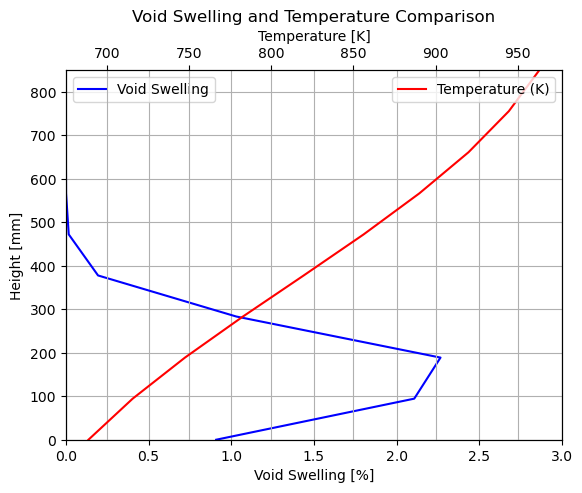
\includegraphics[width=0.8\textwidth]{void_swell.png}
\caption{Cladding swelling due to void formation along the axial direction.}
\label{fig:void_swelling}
\end{figure}
